\chapter{详细设计与实现}

% 本章主要介绍分布式对象存储管理系统中各个微服务的具体实现原理以及数据库的详细设计与实现。
本文将重点阐述分布式数据库的信息处理系统的各个微业务的具体实现原理,及其对系统的详细设置和应用。

\section{注册认证模块设计与实现}

% 认证模块是通过将Spring Security 框架和JWT整合在一起后实现的,Spring Security 是Spring 框架体系中专门处理安全管理方面的框架,它具备功能性强、扩展性高等优点,
% 所以本系统的认证模块采用Spring Security实现。
验证功能是通过把Spring Security框架系统与JWT集成到一起之后完成的,由于Spring Security是Spring框架系统中专用的安全技术的架构,其具备实用性好、扩展度高等特征,所以对该系统的验证功能通过Spring Security完成。

\subsection{用户注册子模块}

% 前端用户的注册请求发送到控制器 RegisterController 中,将来自前端的参数使用QueryVO 类进行封装,前端传递的参数一共有四个:需要
% 注册的角色ID,角色密钥,用户名和密码。在registerUser方法中会调用 Service 层中的方法,该方法与registerUser中的方法同名,且会首先调用该类中judgeTokenByRole
% 的方法,接着调用judgeTokenByRole方法,最后调用insertUserAndRole 方法,judgeTokenByRole 方法将用户传入的角色ID与数据库中的该角色对应的密钥进行比较,如果密钥匹配,则继续执行后续的函数,否则直接返回错误。insertUserInfo方法的主要作用是将用户信息插入到数据库中,但在插入之前需要对用户密码进行编码处理,可以使用Spring Security 框架中PasswordEncoder 接口的实现类BCryptPasswordEncoder对密码进行编码,最后将一条用户角色记录通过 insertUserAndRole 方法插入数据库中,
% 完成用户与角色的绑定。用户注册子模块UML类图如图\ref{fig:用户注册子模块UML类图}所示。

前台发送的参数总共有四种:需要登录的人物ID,角色密钥,账号和密码。且会首先调用该类中 judgeTokenBy-Role的参数,然后使用
judgeTokenByRole方法,再然后使用insertUserAndRole
方式,judgeTokenByRole方式把用户所传入的角色ID和系统中的其他角色所对应的密钥进行了对比,一旦密钥相符,将可以继续执行后
续的函数,或者是返回错误。Inser-tUserInfo技术的主要功能就是把客户数据直接接入到数据库系统中,但是在接入前就必须先对客
户密码进行编号管理,也可以先通过Spring Security框架的PasswordEncoder接口的实现,类bcrypt PasswordEncoder对口令进行
编号,然后再把一个客户角色数据直接通过insertUserAndRole方式直接接入数据库系统中,完成用户与角色的绑定。用户注册子模板
的UML类图如下图五点一中所示。

\begin{figure}[htb]
    \centering
    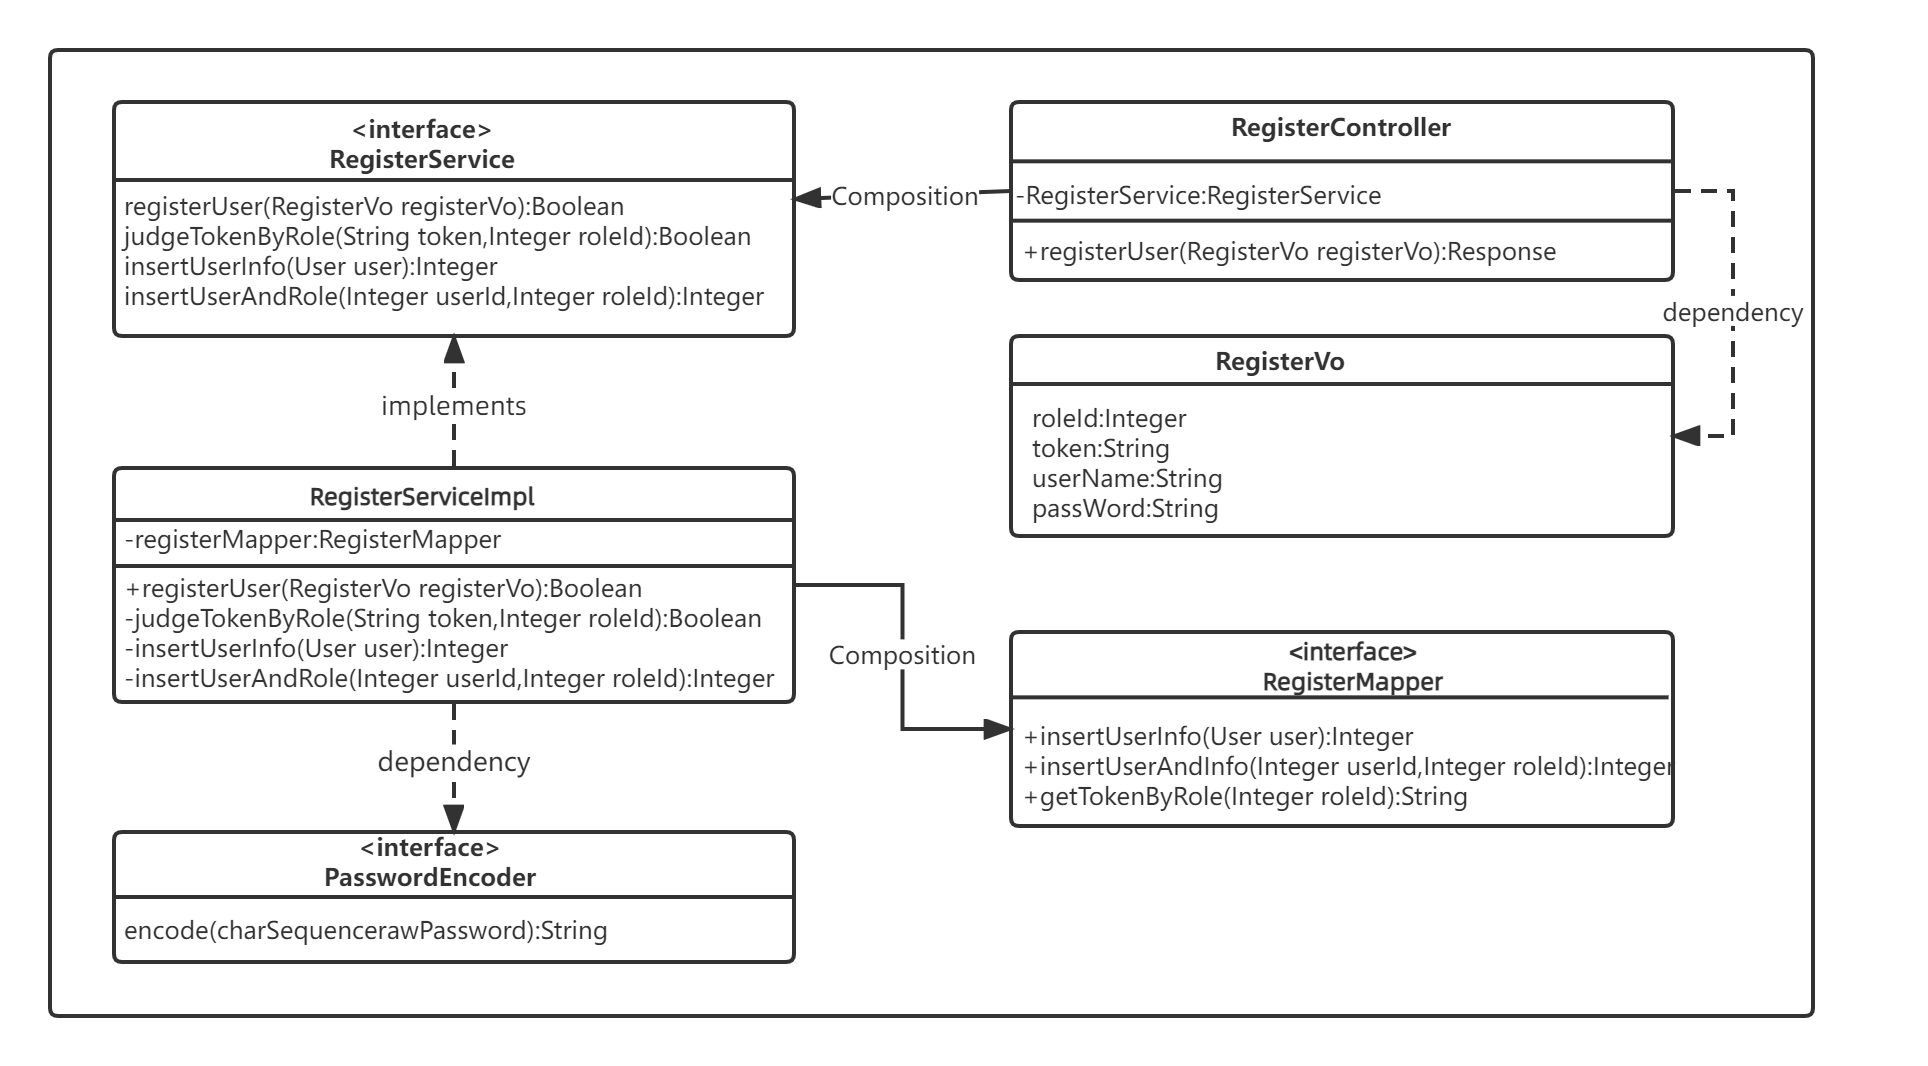
\includegraphics[width=1\textwidth]{my_figures/chapter5/用户注册子模块UML类图.png}
    \caption{用户注册子模块UML类图}
    \label{fig:用户注册子模块UML类图}
%     \note{注:图注的内容不宜放到图题中。}
\end{figure}

\subsection{密码认证子模块}

% 当用户在前端的登录请求到达后端时,其用户名和密码会首先到达过滤器UsernamePasswordAuthenticationFilter中,过滤器将用户名和密码封装成Authentication 对象。
% 过滤器UsernamePasswordAuthenticationFilter内部有一个 attemptAuthentication 方法,该方法会使用ProviderManager 类管理的若干个 AuthenticationProvider 认证提供者去进行认证,包含在DaoAuthenticationProvider 持久层认证提供者中的UserDetailsService 用户细节处理器,该处理器又被自定义的UserDetailsServiceImpl 所 实现,在该方法中可以自定义从数据库中获取用户信息的方法。loadUserByUsername方法也会返回带有用户信息的UserDetails 对象,这里的用户信息是用户的真实信息,而Authentication 对象则是对用户在前端键入数据的抽象, 并不一定与数据库中的信息相匹配。最后,AuthenticationProvider 的 另 一 个 实 现 类
% AbstractUserDetailsAuthenticationProvider 会最终获取到UserDetails 对象,然后由UserDetails 对象调用additionalAuthenticationChecks 方法对去检查用户的密码。

% 密码的校验是通过PasswordEncoder接口的实现类BCryptPasswordEncoder 中的matches方法来完成,该方法会密文进行校验,判断编码格式是否匹配,BCrypt 实体类会进一步
% 完成密码校验的细节。用户名密码认证流程的时序图如图\ref{fig:用户名密码认证流程时序图}所示。

当注册者从前端的注册申请到后端时,其用户名和密码将会首先送到过滤器的UsernamePasswordAuthenticationFilter中,将过滤
器的用户名和密码封装为Authen-tication对象。过滤器 UsernamePasswordAuthenticationFilter 内部有一个 attemp-tAuth
entication 方法,该方法会使用 ProviderManager 类管理的若干个 Authenti-CationProvider层验证提供者可以去进行验证,
包括了在DaoAuthenticationProvider持久层验证提供者中的UserDetailsService用户细节处理器,该处理器后来又被自定义的U
serDetailsServiceImpl所实现,在该技术中可自定义在数据库中提取用户信息的方式。LoadUserByUsername方法也会回到含有用
户消息的UserDetails对象,这图五点一注册登记管理子模型的UML类图里的。最后,AuthenticationProvider的另一个实现类 A
bstractUserDetailsAuthenticationProvider会最终获取到 UserDe-tails对象,然后由 UserDetails对象调用 additionalA
uthenticationChecks方法对去检查用户的密码。

密钥的校验是利用PasswordEncoder接口的实现类BCryptPasswordEncoder中的matches方式的实现,通过这个方式就会密文的校验,
确定编码格式的正确,而BCrypt实体类中可以进一步实现密钥校验的细节。用户名口令验证过程的时序图如图五点二中所示。

\begin{figure}[htb]
    \centering
    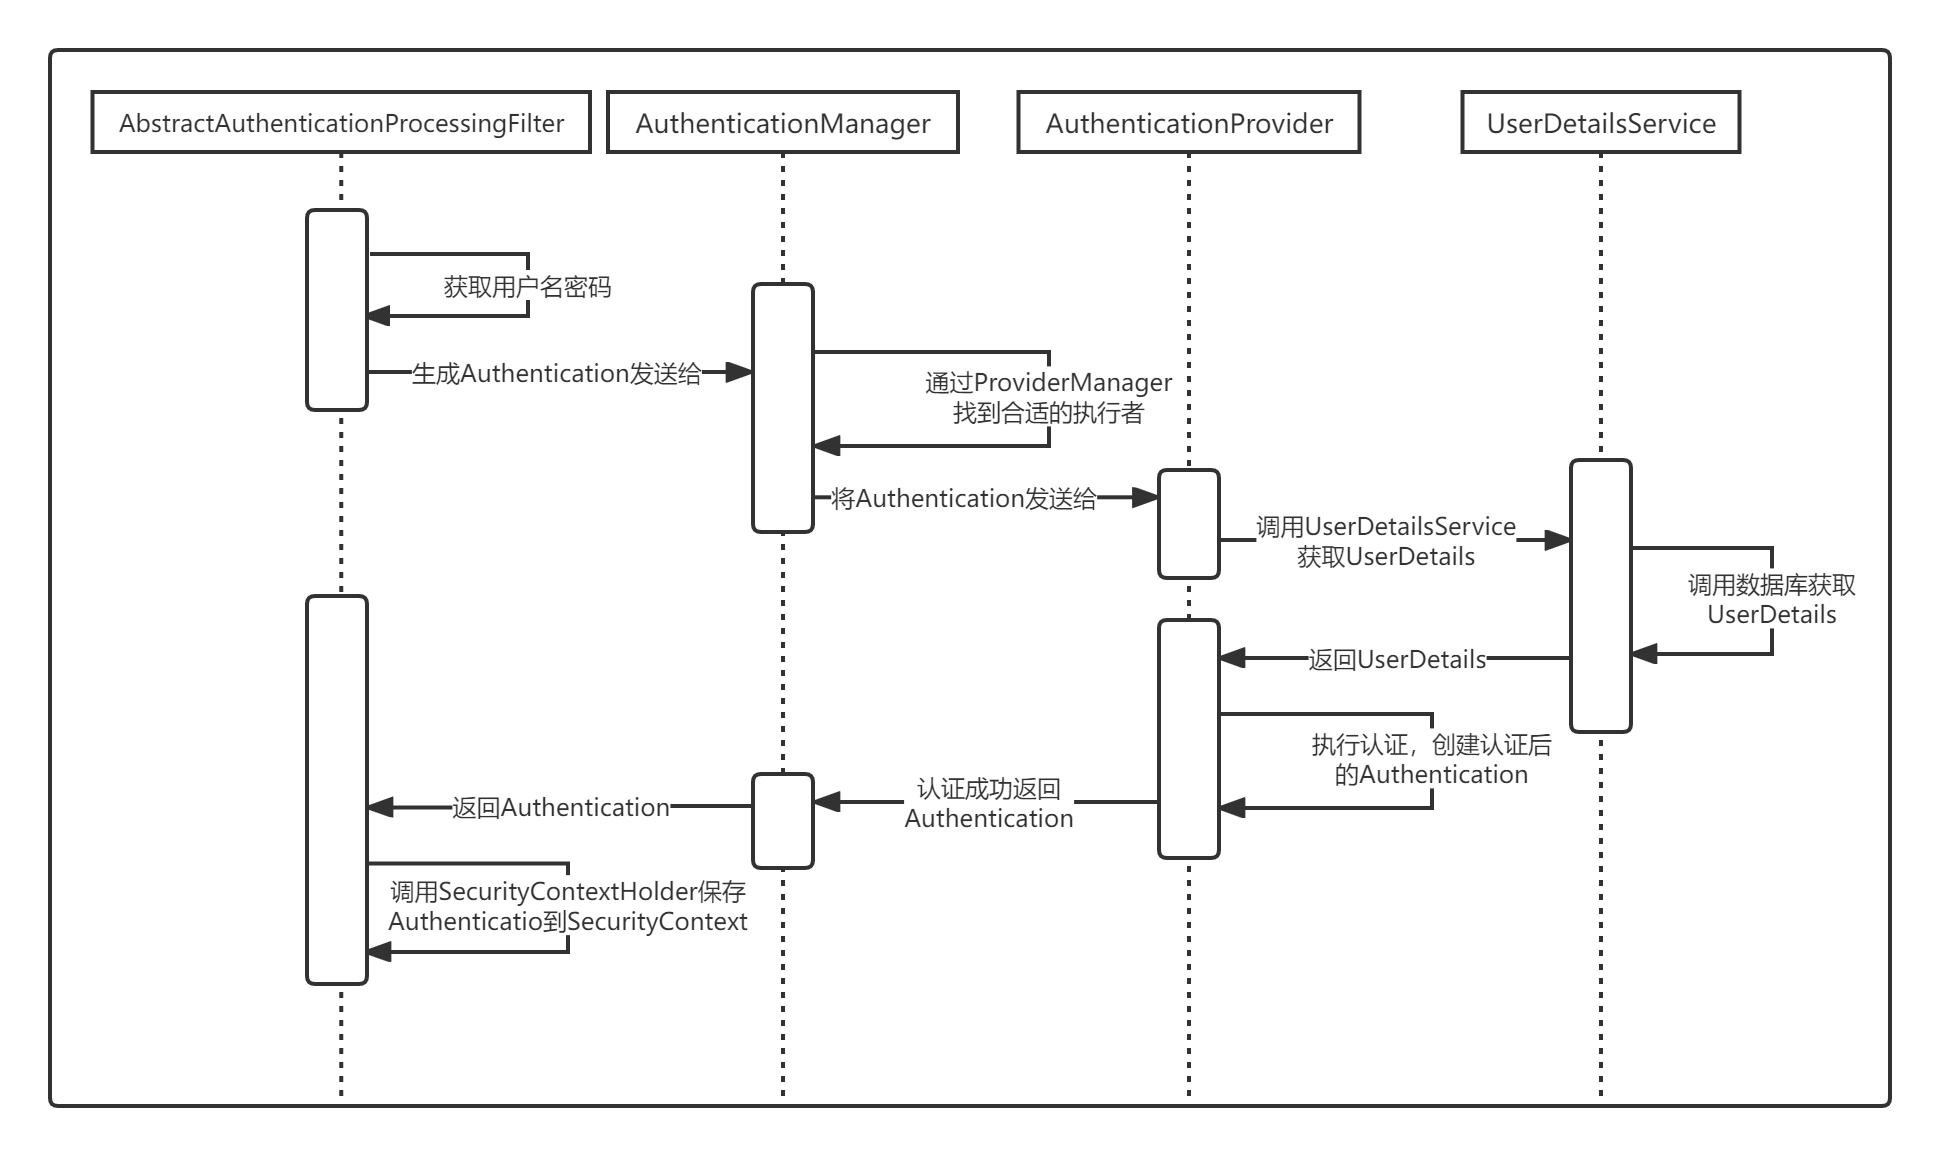
\includegraphics[width=1\textwidth]{my_figures/chapter5/用户名密码认证流程时序图.png}
    \caption{用户名密码认证流程时序图}
    \label{fig:用户名密码认证流程时序图}
%     \note{注:图注的内容不宜放到图题中。}
\end{figure}


\subsection{颁发令牌子模块}

% 上述的UsernamePasswordAuthenticationFilter 类有一个成员变量 :AuthenticationSuccessHandler 类型的 successHandler,在用户的用户名和密码校验成功后,该成员变量可以给该用户颁发token。颁发token的逻辑可以通过实现 AuthenticationSuccessHandler 接口的方式自定义,而token可以根据用户的用户名并通过AuthenticationSuccessHandlerImpl 实现类中的onAuthenticationSuccess 方法调用工具类生成。最后将
% 自定义的 AuthenticationSuccessHandler 与 UsernamePasswordAuthenticationFilter进行绑定。在前面概要设计中已经对具体的 JWT 生成策略进行了阐述,实际的解决方法也被包含在Java的jjwt库中。在使用时,会首先创建一个map集合,需要自定义的对象会存放在该集合中,其中包含用户名和当前时间的键值对,用户名用来对用户进行识别,而当前时间用于对token的过期情况进行判断。该类库构造token的模式是建造者模式,先自定义一个map,

上述的UsernamePasswordAuthenticationFilter类的另一种成员变量:Authenti-cationSuccessHandler类的successHandler
类型,当所有用户的账号和密码都校验完成时,该成员变量才能向其他用户发出token。颁发token的逻辑类可以通过实现Authen-ticat
ionSuccessHandler接口的方法自定义,但token类只能通过用户的用户名并通过AuthenticationSuccessHandlerImpl实现类中的
onAuthenticationSuccess方法调用工具类生成。最后将自定义的 AuthenticationSuccessHandler与 UsernamePass-wordAuth
enticationFilter进行绑定。在前面概要分析中也对具体的JWT生成方法做出了说明,具体的实现方式也都被收录到了Java的jjwt库
中。当调用后,将首先产生一个map集,所有需要自定义的对象都存储在这个集内。

% 然后将创建的token和其过期时间传入map,最后指定签名时使用的算法和密钥。
% 颁发令牌子模块UML类图如图\ref{fig:颁发令牌子模块UML类图}所示。
\begin{figure}[htb]
    \centering
    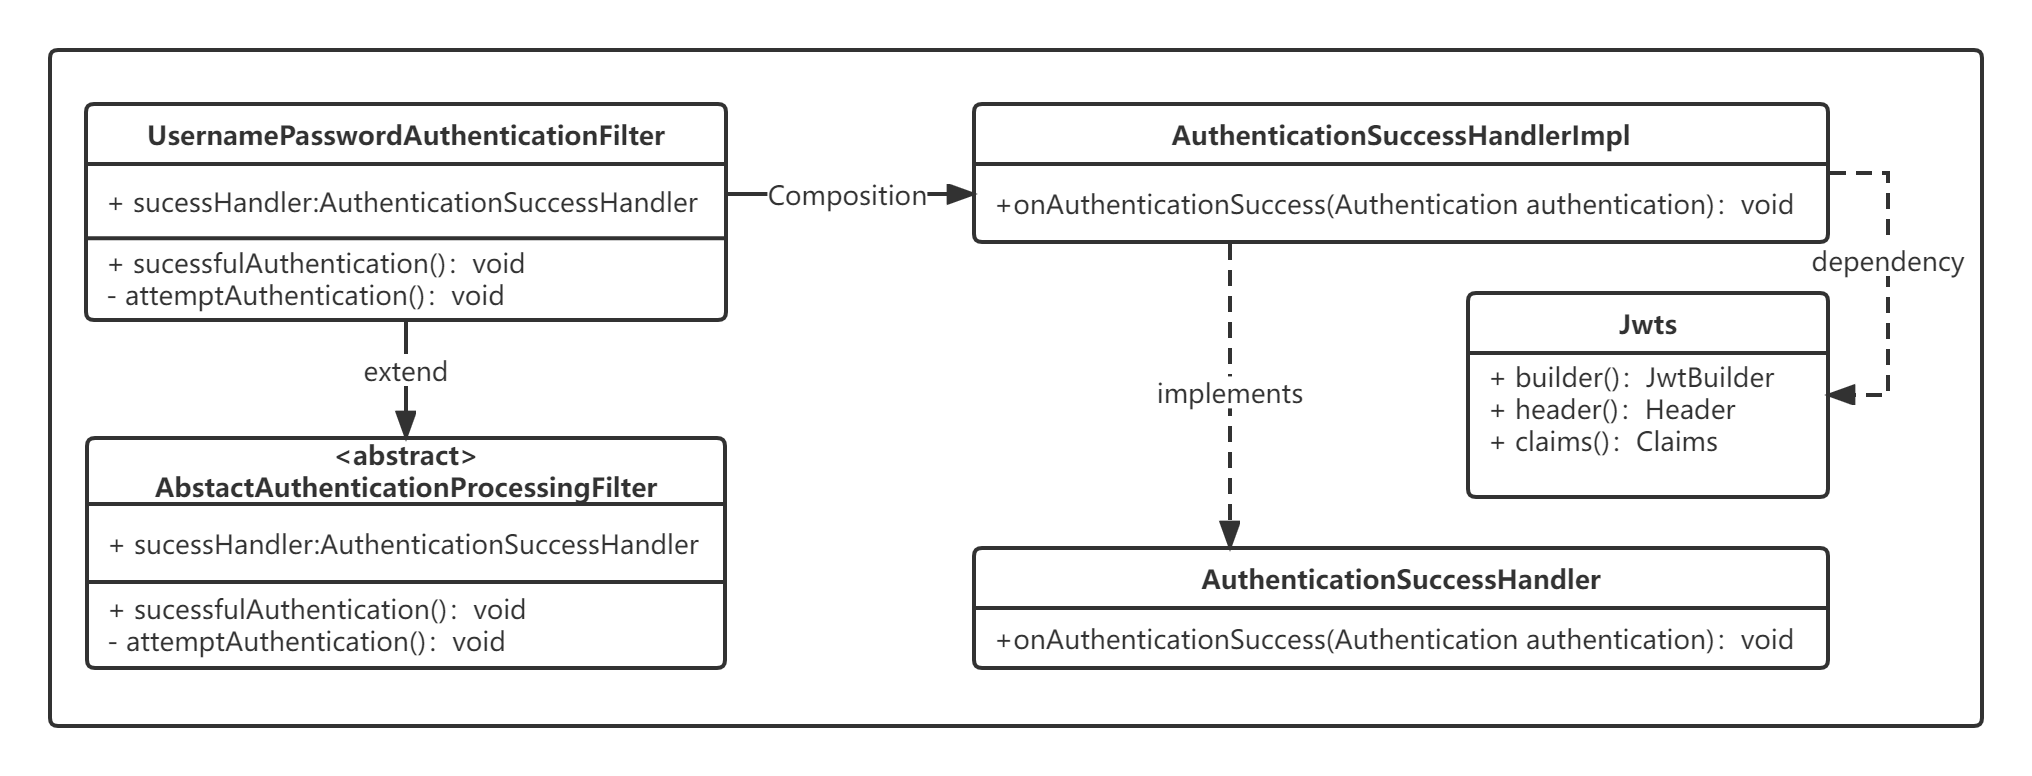
\includegraphics[width=1\textwidth]{my_figures/chapter5/颁发令牌子模块UML类图.png}
    \caption{颁发令牌子模块UML类图}
    \label{fig:颁发令牌子模块UML类图}
%     \note{注:图注的内容不宜放到图题中。}
\end{figure}

\subsection{认证令牌子模块}

% 对令牌的校验是采用在认证微服务的控制层中添加一个接口的方式来实现,该接口首先通过 HttpServletRequest 类型的参数接受请求,在HttpServletRequest 类
% 型的变量中有一个键为 Authorization 的 header,用户附带的token就在这个值中,服务器会使用自己的私钥对token的两部分进行签名,将结果与第三部分进行对比,如果相同,
% 则将创建 token 时定义的 map解析出来,对map中token的颁发时间进行判断,如果颁发时间过期,则向前端返回错误信息提示令牌过期,如果没有过期,则向接口调用者返回用户名,
% 令牌成功认证。该接口不会过滤任何用户,故在Spring Security 的全局配置类中需要给该接口放行。

并将结果和第三部分进行比较,如果一致该接口放行。

\section{网关鉴权模块设计与实现}

% 网关鉴权模块可以分为三个子模块,分别是请求转发子模块,请求鉴权子模块,路由发布子模块。微服务网关是后端的门户,来自前端的所有请求都必须首先经过网关微服务这第一道
% 关卡。网关模块处理来自前端请求的时序如图所示。

网关的鉴权功能主要包括三个种子功能,分别为申请转发子模块,请求鉴权子模块,以及路由与转发子模块。微服务网关是最后端的关口
,因此来自前端的任何申请都需要事先通过网关微服的第一道关卡。网关模块接收来自前台所有申请的时序,如图所示。

\subsection{请求转发子模块}

% 路由是网关的基本单元,其配置项如表所示。在此模块中,使用请求Path校验条件谓语将- Path=/gasweb 和- Path=/OAuth 等内容填写在配置文件中,内置的 PathRoutePredicateFactory 
% 类会在框架启动时对请求路径进行正则匹配。

% 在此模块中配置四组路由,第一组路由的URI 设置为认证微服务的 URI,Predicate 设置为- Path=/OAuth,该路由表明将请求转发至认证微服务,这组路由不需要设置路由器。
% 第二组路由的URI设置为策略控制模块的URI,即将该请求转发至策略控制模块, Predicate 为- Path=/policyweb。第三组路由的URI设置为文件存取模块的URI,即将该请求转发至文件存取模块, Predicate 为- Path=/filewe。
% 第四组路由的URI设置为系统维护模块的URI,即将该请求转发至系统维护模块, Predicate 为- Path=/systemweb。对这三组应用自定义的过滤器 JwtCheckGatewayFilter,
% 即访问目标为这三个微服务的请求需要经过各种限制才可访问。

% 此模块的主要工作是在 Spring Boot 的配置文件中配置与路由有关的信息, 无相关的实现类, 但此模块是网关微服务最基础和核心的功能, 因此将它单独作为一个子模块。

路由是系统的基础组成部分,其配置项如下图所示。

在此模型中设置了四队路由,第一集团路由的才可以访问。

该功能的主要任务是在Spring Boot的系统配网关微功能的基本和关键的特性,所以可以把其简单地当成一个子功能。

\begin{center}
    \renewcommand\arraystretch{1.5}{
    \setlength{\tabcolsep}{5mm}{
	\begin{longtable}{|p{2cm}<{\centering}|p{10cm}<{\centering}|}
		\caption{Spring Cloud Gateway路由配置项说明表}\label{Spring Cloud Gateway路由配置项说明表}\\
		\hline
        \bf{属性} & \bf{解释说明} \\
        \hline
        ID & 路由ID\\
        \hline
        URI & 转发到目的地址的URI\\
        \hline
        Predicate & 路由与转发的判断标准,可通过所请求的Path、Method、Header<br>等标准实现转发 \\
        \hline
        Filter & 也可以为请求应用配置接修改,但也可不配置过滤器。\\
        \hline
	\end{longtable}}}
\end{center}

\subsection{请求鉴权子模块}

% 在第二、三、四组路由的过滤器中会对请求进行鉴权,以文件存取模块为例,该过滤器首先会获取该用户请求文件存取模块的认证令牌,该认证令牌在HTTP 请求header 中的
% Authorization字段中,接着以该令牌作为参数去访问认证模块的接口check-token,该接口对网关提供的令牌进行解析,如果解析成功,令牌中用户的用户名会被网关获取到,
% 如果解析失败,客户端会收到来自网关的错误信息。所以此次解析主要是达到验证令牌正确性和获取令牌中用户的用户名这两个目的,验证令牌的正确性是为了防止令牌被篡改、
% 伪造或超过有效时间,获取用户名是为了方便获取该用户的权限列表。最后获取该请求的URI, 在权限列表中寻找该URI,如果能找到,则说明有访问权限,由路由转发至文件存
% 取微服务,如果不能找到,则前端会收到无权限的错误信息。请求鉴权子模块的时序图如图\ref{fig:网关接收请求时序图}所示。
而一旦分析失败,则客户端就会接受来自网
关的错误信息。所以此次解析主要为达到了验证令牌准确性,以及获得了令牌中用户的账号这二个目的,检验令牌的准确性主要是为了避
免令牌被人修改、被盗用或者超出了有效时限,而获得账号则是为了便于得到该用户的权限列表。最后读取了该请求的URI,从权限表中
搜索该URI,如果被发现,则表示有访问权限,可以通过路由转发或文件存取微服务,如果没有发现,则前端将接受未授权的出错报告。请
求鉴权子模块的时序图如图五点四所示。

\begin{figure}[htb]
    \centering
    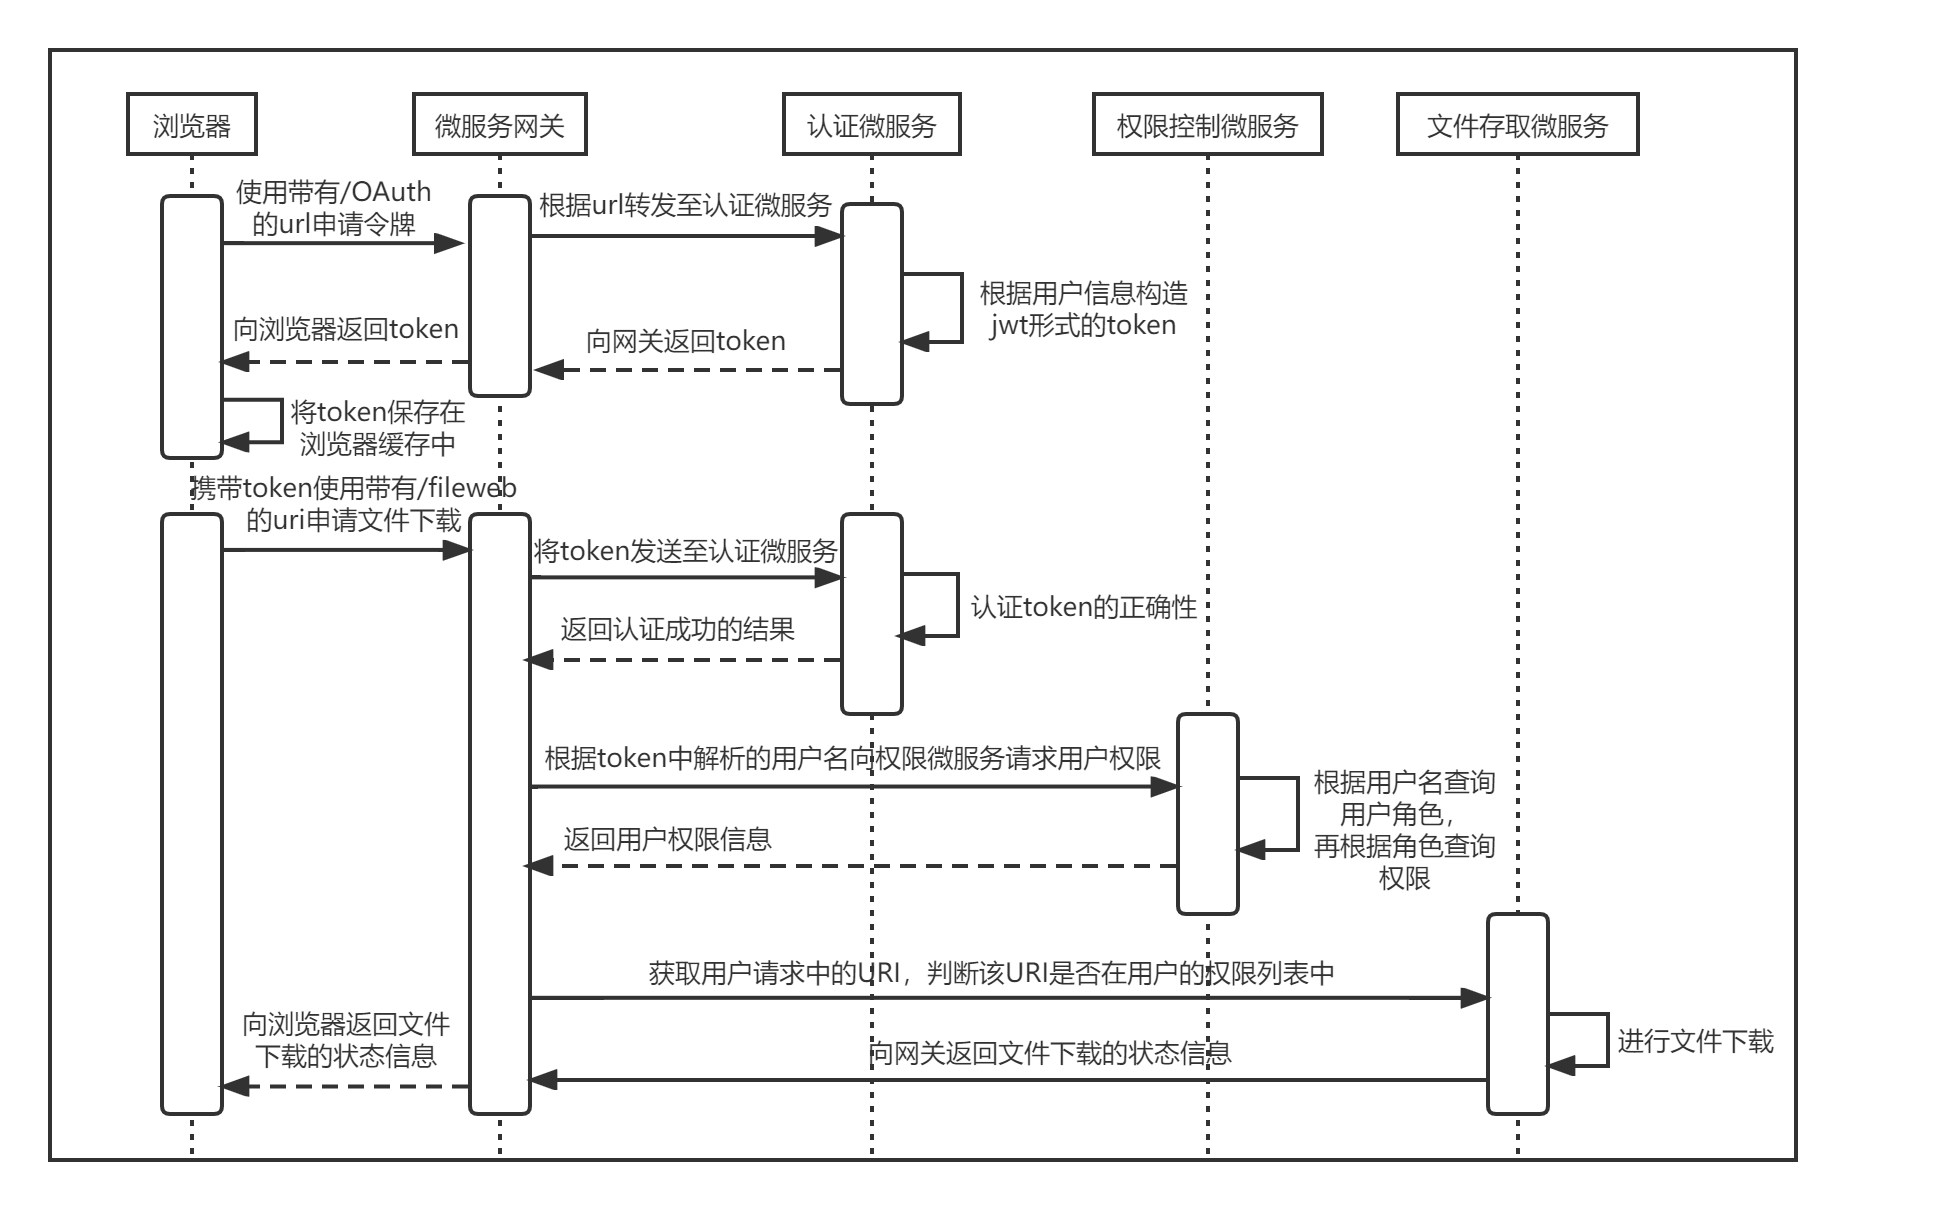
\includegraphics[width=1\textwidth]{my_figures/chapter5/网关接收请求时序图.png}
    \caption{网关接收请求时序图}
    \label{fig:网关接收请求时序图}
%     \note{注:图注的内容不宜放到图题中。}
\end{figure}

\subsection{路由发布子模块}

% 传统的网关服务在对配置文件中的路由信息进行修改之后,整个系统需要重新上线,这种做法在实际生产中是不可接受的。因此,在现在的实际工程中,采用的是动态网关的策略。
% 将写在配置文件中的信息进行抽象,然后和网关框架提供的接口一起进行动态组装,封装成一个RouteDefinition 对象,以此实现在不中断服务的情况下发布新路由。如果只是
% 简单的对这些接口进行调用后发布,重启后仍然会出现网关信息丢失的问题,所以对于待发布的网关信息在调用前就需要进行持久化,但考虑到网关需要保持单一职责的设计原则,
% 这部分功能放在权限控制模块中去完成,因为权限控制模块只有管理员才有操作权限,符合单一职责的设计原则。简单的持久化操作和调用接口虽然可以完成需求,但是由于这两个
% 模块具有较高的耦合度,权限控制模块在发送了请求后,可能会出现网关服务不可用从而导致请求丢失的问题,此时用户端对此却一无所知。

% 为了解决这个问题,考虑加入了消息中间件,当网关服务不可用时可将请求保存在消息中间件中,等到网关可用时去消费中间件里的消息并发布路由。由于通信量不大,这里采用的
% 是Redis作为两个模块之间通信的桥梁,主要是使用Redis中的List数据类型来实现消息队列。Redis可以通过POP指令向从队列获取元素,通过PUSH向消息队列添加元素。网关模块
% 可以通过定时任务从消息队列中获取消息,即执行POP命令从队列中取元素,但由于大部分时间队列为空,定时任务的时间也不好确定,定时任务时间间隔太长,可能会造成消息队
% 列中的数据长时间得不到处理,定时任务时间间隔太短,可能会出现忙等而浪费CPU资源。

% Redis还提供了阻塞式拉取信息的命令BRPOP,权限控制模块作为生产者,使用LPUSH推送一条消息,网关鉴权模块作为消费者,使用BRPOP接收一条消息。当队列为空时,该线程的
% 任务会发生阻塞,这样就可以避免循环检查数据是否存在。当权限控制模块将网关的相关信息推送至消息队列时,会唤醒网关鉴权模块阻塞的任务,获取Redis中的信息,并将其封
% 装成RouteDefinition 对象,然后发布在内存中。采用这种方案,可有效缩短定时任务的执行时间间隔,定时任务会之间会严格同步,节省CPU资源。路由发布子模块的时序图如
% 图\ref{fig:路由发布时序图}所示。


传统的网关服务在需要对配置文件中的路由数据进行调整以后,整个服务就必须重新上线,这种做法在实际生产中是不可接受的。所以,在现在的实际工程中,使用的都是动态网关的策略。把写入到配置文件中的消息进行了抽象,然后再与网关框架中提供的接口一起进行了动态组装,并封装为一个RouteDefinition对象中,但同时考虑了系统必须具有一个职能的设计原理,将这些职能都放到权限控制模块中才能实现,而由于权限管理功能只有用户才有使用权限,必须遵循单一职能的设计原理。简单的持久化功能和调用接口虽然能够实现需求,不过因为这二种功能存在很大的耦合性,用户管理功能在发出用户申请时,也容易产生网关服务不能用而造成申请丢失的问题,此时用户端对此却一无所知。

为处理这种问题,考虑加入了消息中间件公司,在网关服务不能使用时可把请求存储到消息中间件中,在等待网关服务
使用时去消费消息中间件公司里的消息并发送路由。但因为通信量不大,所以这里使用的是Redis作为二个模块之间
联系的桥梁,主要是通过Redis中的List数据模式来完成消息队列。但是因为大多数时候组队为空,所以定时任务的持续时间并不好判断,如果定时任务时间间隔过长,很可能会导致消息队列中的信息长期不能处理,如果定时任务时间间隔太短,可能会出现忙等而浪费 CPU资源。

而通过这个方法,就可以有效减少了定时任务的运行时间间隔
,定时任务会之间会严格同步,节省 CPU资源。路由发布子模块的时序图如图5.5所示。

\begin{figure}[htb]
    \centering
    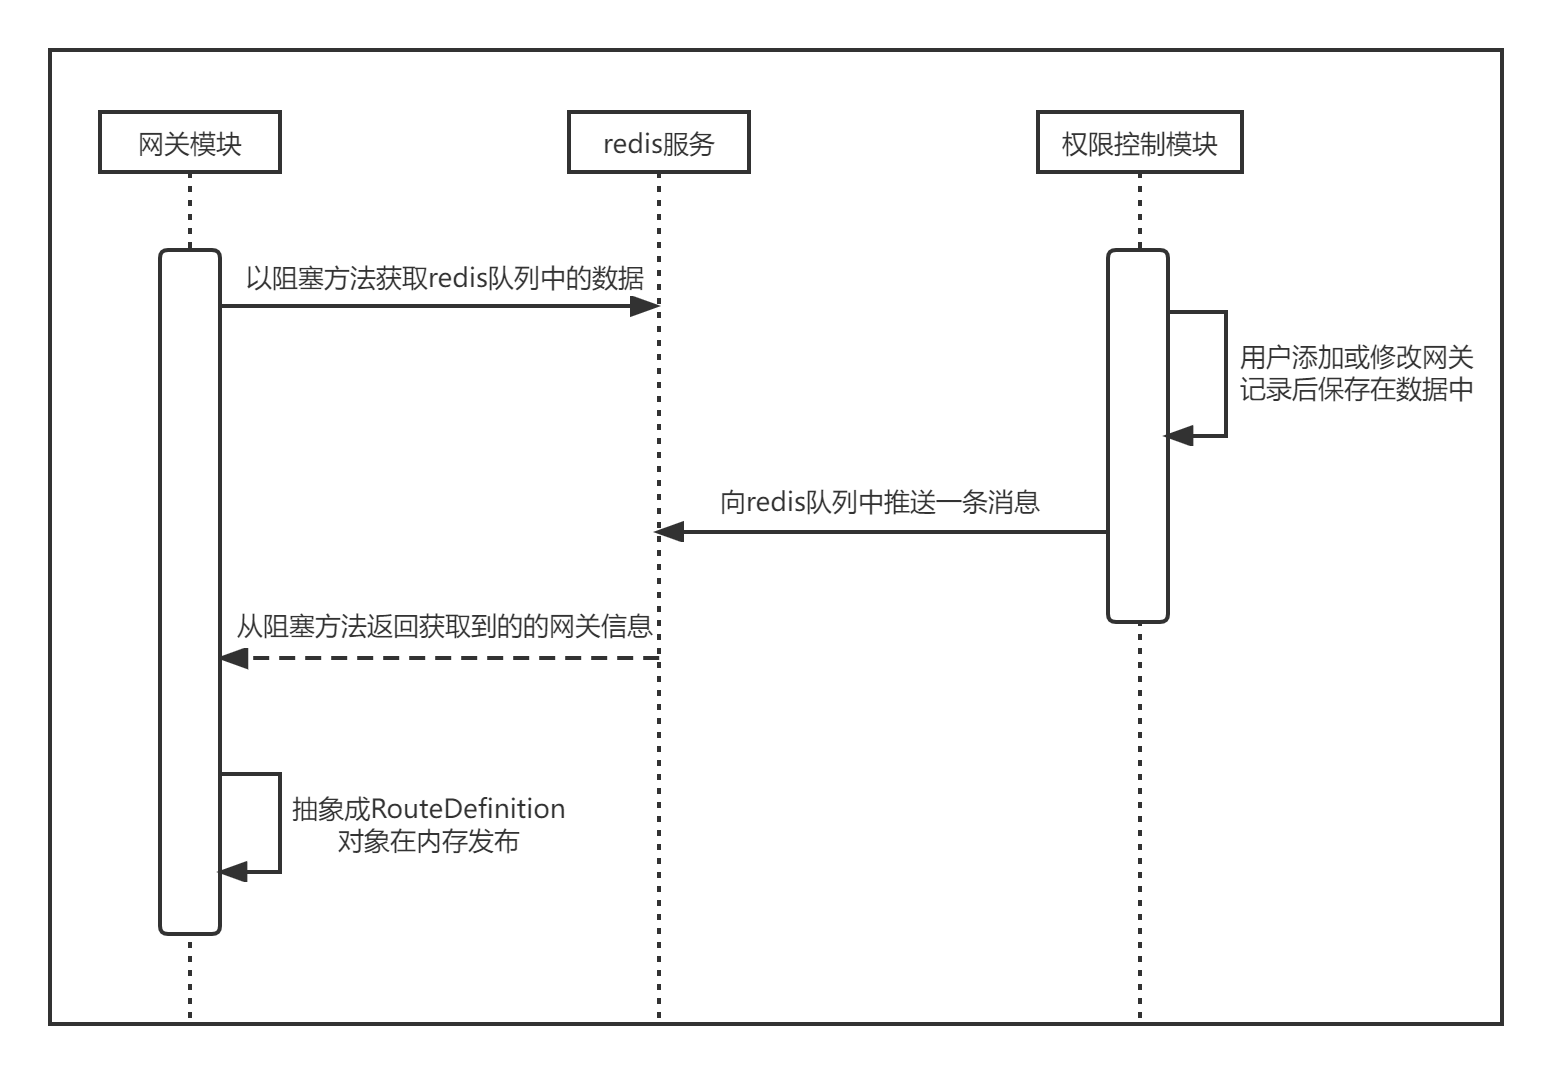
\includegraphics[width=1\textwidth]{my_figures/chapter5/路由发布时序图.png}
    \caption{路由发布时序图}
    \label{fig:路由发布时序图}
%     \note{注:图注的内容不宜放到图题中。}
\end{figure}

\section{权限控制模块设计与实现}

\subsection{用户角色权限管理子模块}

% 该模块一共管理三个对象,分别是用户,角色和权限。由于三种对象的管理方式基本相同,所以将它们归为一个子模块。系统中默认的角色一共有三种,分别是超级管理员,普通
% 管理员和普通用户。如果有需要,管理员可以在后端管理系统中添加新角色或修改已有角色,但不可对默认角色进行修改或删除的操作。系统中的权限实际上是指是否含有访问某
% 个系统接口的路径URI,每条访问路径就是一个权限,用户需要拥有什么权限就由管理员手动添加相关路径,其中普通管理员的权限由超级管理员进行配置。

% 权限控制模块中的添加、删除、修改、查看操作最后会对应到数据中的INSERT、DELETE、UPDATE、SELECT操作,这些操作主要涉及的数据库表有:用户表、角色表、权限表。
% 以角色对象为例,角色对象的类图如图\ref{fig:用户角色权限子模块UML类图}所示。

这个模型一共管理了三种对象,依次为用户,角色和权限。因为三种类型的控制方法都相同,所以可以把它归于一个子模型。操作系统中默认的客户一共有三种,顺序为超级管理员用户,正常客户和一般客户。但如有特殊需求,客户也可在后端管理中增加新人物或更改现有人物,但不可对默认角色进行修改或删除的操作。操作系统上的授权实际上是指定是否存在使用特定操作系统连接的路径URI,每一条的路径就是一条权限,用户需要拥有什么权限就由管理员手动添加相关路径,其中普通管理员的权限由超级管理员进行配置。

权限管理模型中的新增、移除、更改、查看等操作,最后都会对应到数据中的IN-SERT、DELETE、UPDATE、SELECT等操作,而这些操作中主要涉及的数据库表有:用户列表、角色表、权限列表。以人物对象为例,人物对象的类图如图五点六所示。

\begin{figure}[htb]
    \centering
    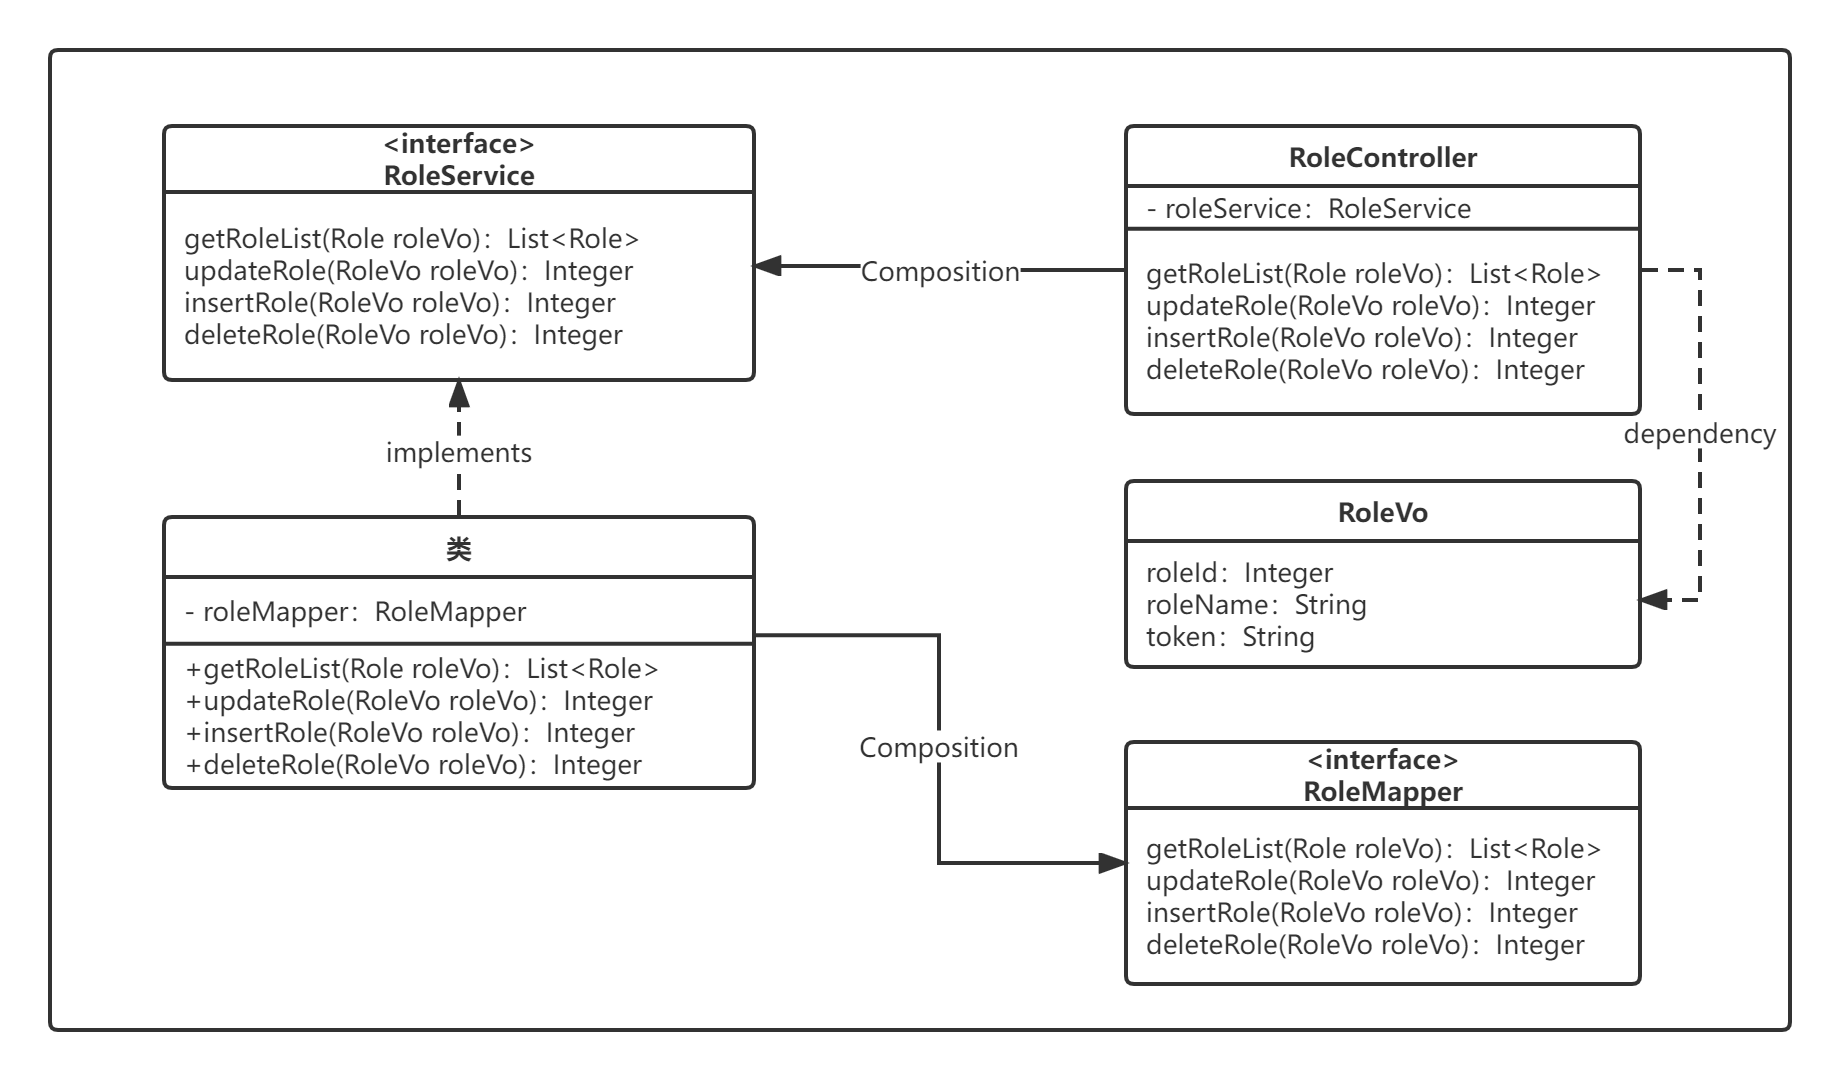
\includegraphics[width=1\textwidth]{my_figures/chapter5/用户角色权限子模块UML类图.png}
    \caption{用户角色权限子模块UML类图}
    \label{fig:用户角色权限子模块UML类图}
%     \note{注:图注的内容不宜放到图题中。}
\end{figure}
 
\subsection{角色分配子模块}

% 该模块主要是将账号、角色和权限这三个对象关联起来,将用户与角色进行绑定,将角色与权限进行绑定。实现这两个操作的原理高度相同,以将权限分配给角色的操作为例,系统
% 中的角色数量与权限数量相比要少很多,因此角色与权限之间是一对多的关系,即一个角色可能对应多个权限。每个角色都关联了一个分配按钮,会看到包含所有权限的列表,该
% 角色已分配的权限会被标记,未分配该角色的权限点击后可以进行分配角色的操作,已分配点击后可以取消分配,最后点击保存可以保存修改。实际原理是前端将正在分配中的角色
% 编号和所有选中的权限编号发送给后端,后端根据角色编号将出现在角色权限关联表中的所有记录删除,再根据权限编号集合,将这若干条记录插入该表,由于需要先删除在插入,
% 所以在Service层进行事务控制,任何一步出现错误,数据库都会进行回滚。以角色权限分配为例,角色权限分配的类图如图\ref{fig:角色分配子模块UML类图}所示。

该模块主要是将账号、角色和权限这三个对象关联起来,将用户与角色进行绑定,将角色与权限进行绑定。实现这二种功能的原则高度
一致,以把权力划分到角色的操作为例,系统中的人物总量和权力总量相对要小许多,所以人物和权力之间有相对多的联系,即一个人物
可以对应多种权力。每个角色都关联了一个分配对象,可以得到包含了权力的列表,每个人物所分享的权力都有记录,所分享该人物的
权力点击后才能完成分配对象的操作,已分配点击后才能解除分配,最后点击保存才能保存修改。具体原理是前台把正在配置中的角色
名称以及所选中的权限编码传给后端,后端按照角色名称把出现在角色授权关系表上的所有信息删掉,然后按照授权编码集合,把这若干
个信息接入该表,因为需要先删后接入,所以需要Service层实现事务管理,任何一步出现错误,数据库都会进行回滚。以角色权限分配
为例,角色权限分配的类图如图5.7所示。

\begin{figure}[htb]
    \centering
    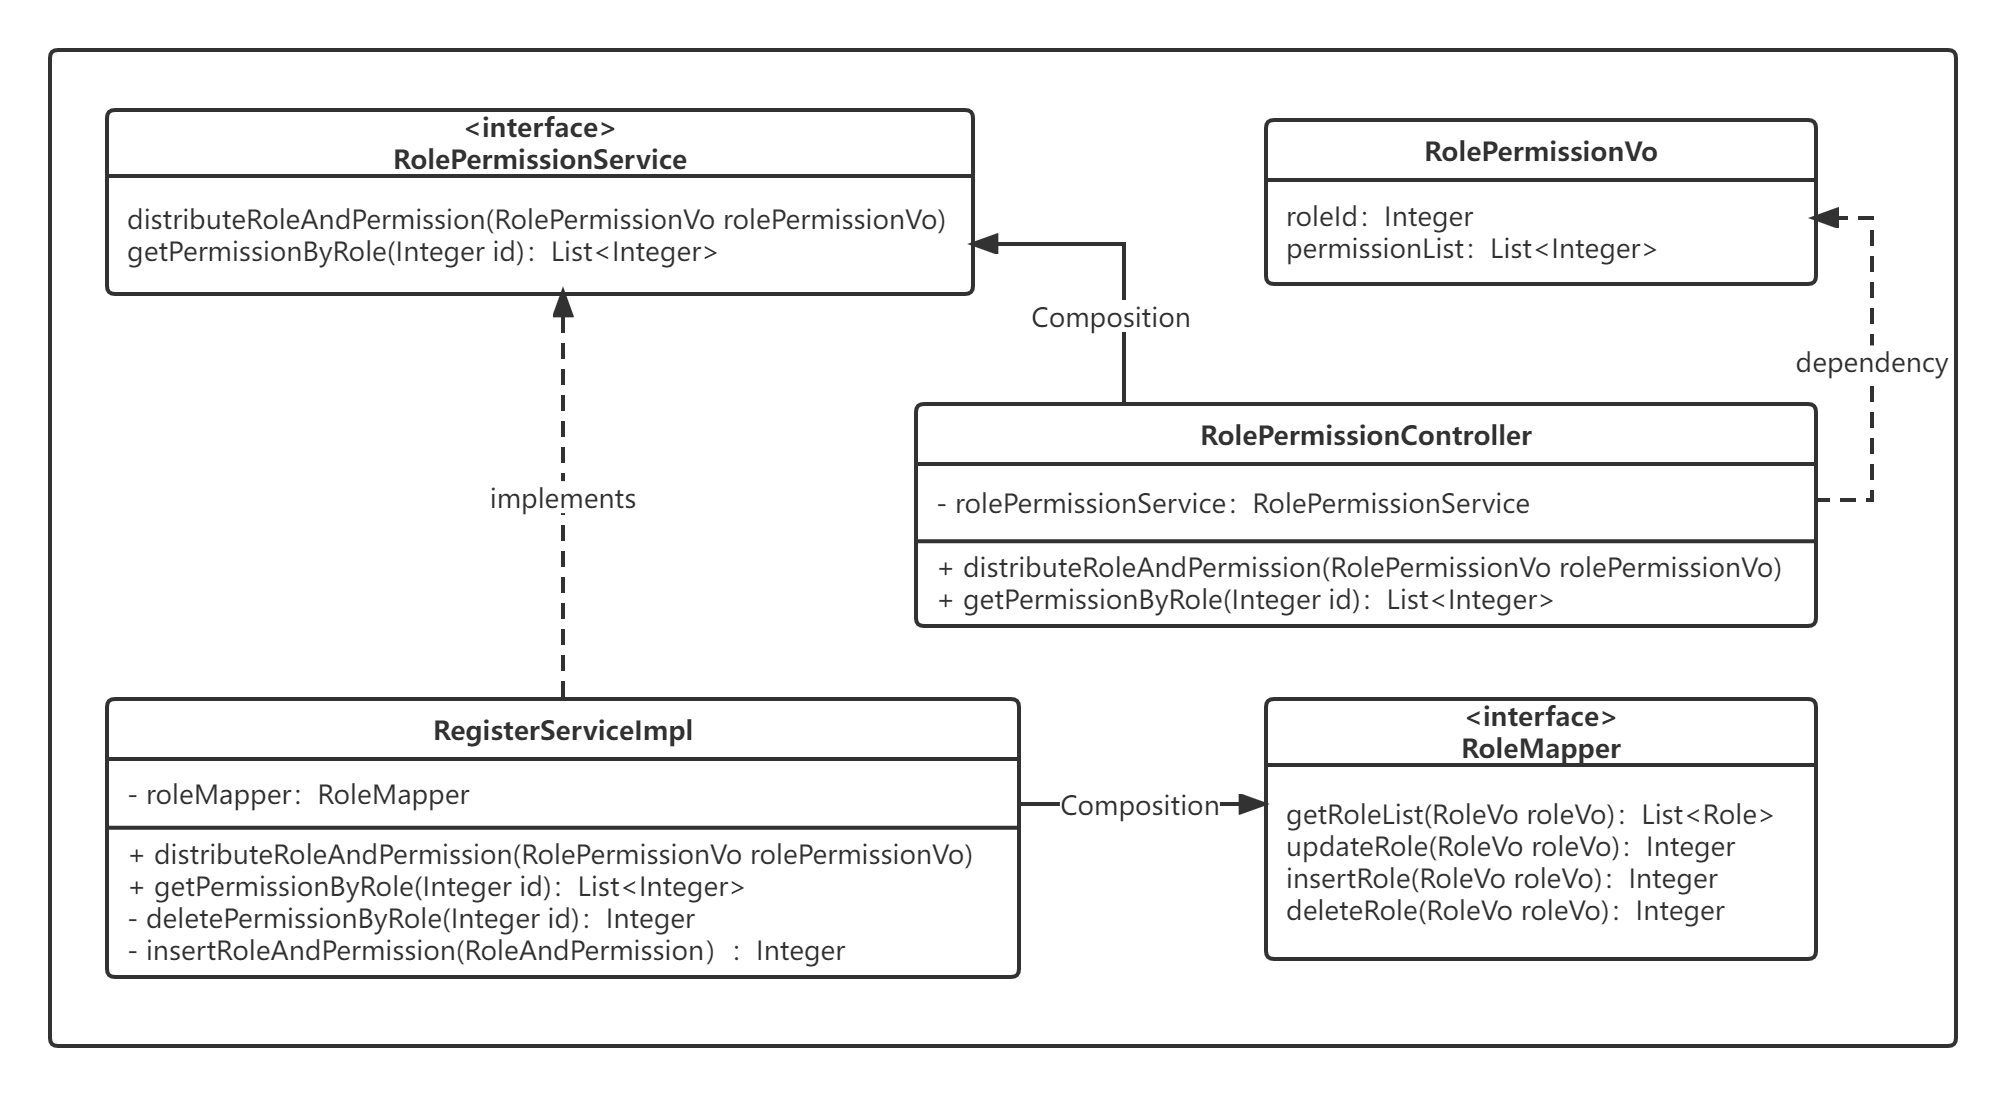
\includegraphics[width=1\textwidth]{my_figures/chapter5/角色分配子模块UML类图.png}
    \caption{角色分配子模块UML类图}
    \label{fig:角色分配子模块UML类图}
%     \note{注:图注的内容不宜放到图题中。}
\end{figure}

\subsection{网关路由管理子模块}

% 网关路由管理主要负责协助网关鉴权模块动态发布网关功能的实现,对于Redis消息队列而言,它充当生产者的角色。管理员可以对已有的路由信息进行新增、删除和修改的操作,
% 路由的基本信息由ID、URI、一组Predicate和一组Filter组成。管理员输入这些信息后,点击保存按钮即可将其保存到数据库中,最后点击发布按钮,即可将更改的需求推送到
% 消息队列中,然后会唤醒阻塞的网关模块,完成路由的更新操作。

网关路由管理功能主要是为了协助网关鉴权系统动态的管理网关功能的实现,对Redis消息队列系统来说,主要扮演生产者的作用。
管理者也能够对现有的路由数据作出新建、撤销或者更改的动作,路由的基础数据由ID、URI、一个Predicate,以及一个Filter
所构成。当管理者选择了这些数据之后,通过单击储存按键就可以直接将资料储存在信息库中,然后再单击消息发布按键,就可以
将更改的信息发布在消息队列中,并且还可以提示阻塞的消息网关<br>图五点七角色分配子单元的UML类图模块,完成路由的更新操作。

\section{策略控制模块设计与实现}

\subsection{用户分组管理子模块}

该模块管理用户和分组两个对象。由于两种对象的管理方式基本相同,所以将它们归为一个子模块。这里的用户和分组指的是存储服务器上注册的用户和分组,和存在数据库里的用
户信息有一些区别。存储用户信息主要反映的是用户存储相关的信息,如申请的存储容量、上传的文件数、创建的Bucket数等信息,这些信息都是从存储服务器上获得的实时信息,
分组也是对存储用户进行分组,且分组只能有存储服务器上注册的管理员才有权限创建、修改和删除。以用户对象为例,用户对象的类图所示。

\subsection{策略管理子模块}

策略管理主是对存储用户的访问策略进行管理。系统中的策略主要分为Bucket访问策略和用户访问策略。Bucket访问策略主要有public、custom和private三种,系统内置的用户访问策略主要有五种,分别是控制台管理员(consoleAdmin)策略、
诊断(diagnostics)策略、只读(readonly)策略、读写(readwrite)策略和只写(writeonly)策略。这些都是系统内置的策略,对于这些策略只能进行查看,不能进行修改或
删除操作。如果有需要,管理员可新增自定义的策略,在新增策略时,管理员需要输入新增策略的具体内容,在后端会形成json文件,然后作为参数传入相关创建策略接口,对于新增
的策略,管理员可以对其进行修改、删除和查看操作。策略管理的类图如图所示。

\subsection{策略分配子模块}

该模块主要是将用户、分组和策略这三个对象关联起来,将用户与分组进行绑定,将用户与策略进行绑定,将分组与策略进行绑定。实现这些操作的原理高度类似,以将策略分配给
用户为例,用户和策略是一对一的关系,每个用户只能拥有一个访问策略。每个用户都关联了一个策略分配按钮,下拉菜单可以看到所有的策略,选择其中一个策略后,并点击确认
分配,则将该策略与该用户进行绑定。当然,对于策略分配还涉及到Bucket的访问策略,该部分在桶管理模块实现,Bucket的访问策略由用户自己设定,只能设置为内置的三种:
public、custom、private,后续用户对Bucket的访问由用户策略和Bucket的策略共同决定。当设置Bucket的使用方式是public后,用户必须不通过任何验证才能进行使用资源;
当设置Bucket的访问方式是custom时,Bucket的最终访问策略由具体的用户访问策略决定,用户访问策略可以是系统内定的策略,如只读(readonly)策略、读写(readwrite)策略和
只写(writeonly)策略,也可以是自定义的访问策略;当设置Bucket的访问策略为private时,用户未经授权不能进行任何操作,所有用户访问策略失效。因此,Bucket的访问策
略权限要大于用户访问策略。

\section{文件存取模块设计与实现}

\subsection{桶管理子模块}
% 该模块主要是对文件桶进行管理。主要是进行创建、删除、修改、查看和策略分配的操作。但操作的前提是用户拥有对应的访问策略,比如用户对桶的访问策略是只读,
% 那么该用户将只能对桶进行查看,无法进行修改、删除等其他操作。对桶进行删除操作时,需要在桶里的文件全部被删除之后方可进行,即只可删除空桶。这里的用户不仅指普通用户
% ,还包括普通管理员。在对桶进行非创建操作时,需要先判断桶是否存在,如果桶不存在,则向前端反馈错误信息。这些操作也是直接作用在存储服务器上,不会与数据库产生交互。

该模块主要是对文件桶进行管理。主要是进行创建、删除、修改、查看和策略分配的操作。但操作的前提是用户拥有对应的访问策略,
比如用户对桶的访问策略是只读,那么该用户将只能对桶进行查看,无法进行修改、删除等其他操作。对桶进行删除操作时,需要在桶里
的文件全部被删除之后方可进行,即只可删除空桶。这里的用户不仅指普通用户,还包括普通管理员。当对木桶进行非创建性操作时,必
须首先确定木桶是否存在,若桶不存在,将向前端反馈错误的信息。这些操作也是直接作用在存储服务器上,不会与数据库产生交互。

\subsection{文件上传子模块}

% 文件上传模块主要负责将用户的文件上传至数据存储服务器中,支持上传多种不同类型的文件,也可以进行多文件批量上传。上传时后端会通过客户端Client向存储服务器发送查询桶
% 的命令,判断文件桶是否存在,主要是防止前端显示和存储服务器没有同步的情况,避免发生错误。上传时前端会显示正在上传的进度条和上传的带宽,用户可以暂停上传或取消上传。
% 如果遇到网络断开的情况,文件上传的过程会显示上传失败,用户可以等待网络恢复后,继续上传。
文档上传功能主要是将客户的文档提交至文件存放服务器上,能够提交多种不同形式的文档,并且能够实现多文件批量提交。上传时后端
会通过客户端Client向存储服务器发送查询桶的命令,判断文件桶是否存在,主要是防止前端显示和存储服务器没有同步的情况,避免发
生错误。上传时前端会显示正在上传的进度条和上传的带宽,用户可以暂停上传或取消上传。如果遇到网络断开的情况,文件上传的过程
会显示上传失败,用户可以等待网络恢复后,继续上传。

\subsection{文件下载子模块}
文件下载模块主要负责将文件从数据存储服务器下载到用户本地。和文件上传一样,也支持多文件批量下载。下载时后端会通过客户端Client向存储服务器发送查询桶
的命令,判断文件桶是否存在,主要是防止前端显示和存储服务器没有同步的情况,避免发生错误。在下载过程中前端可以看到文件下载的实时进度,如果遇到网络波动或
断线,前端会有相应的反馈通知,网络故障时,系统会暂停文件的下载。整体的操作流程和文件上传类似。

\subsection{文件删除子模块}
% 文件删除模块主要负责对用户Bucket中的文件进行在线删除。这里对文件的删除操作其实是直接将文件从数据存储服务器中删除,支持多文件批量删除,删除是会提示前端进行确认,
% 因为删除操作是不可逆的。

文件删除模块主要负责对用户 Bucket中的文件进行在线删除。这里对文件的移除动作其实就是直接把文件从数据存放服务器中移除,
支持对多文件批量移除,但移除时是会提醒前端进行确认工作,因此移除动作是不可逆的。

\section{系统维护模块设计与实现}

\subsection{服务器管理子模块}
服务器管理模块主要负责对存储服务器进行启动和停止以及对服务器相关信息进行查看。该模块主要是方便运维人员对存储服务器进行维护,运维人员可以很方便在系统内对存储服务
进行停机、启动或重启的操作,也可以很直观的查看到存储服务器当前的信息,比如服务器版本、网络状况、已用容量、可用容量等信息。服务器管理活动图如图所示。

\subsection{集群管理}
集群管理模块主要负责对服务器集群进行扩容、清理以及对集群状态进行查看。AliIO支持集群的直接扩容,在准备好准备扩充的另一个集群后,只需要在系统中输入集群的相关信息,
然后点击扩容即可,但是扩容之后需要重启当前扩容的集群才可生效。集群清理相当于将当前集群进行禁用,点击集群清理后同样需要重启集群方可生效。

\subsection{日志管理}
日志管理模块主要负责对平台日志和存储日志进行管理。主要是对日志信息进行查看和删除操作。平台日志指的是用户登录管理平台后所进行的一些操作信息,存储日志是用户与存储
服务器进行交互后产生的一些操作信息,比如上传文件、删除文件等操作记录。平台日志主要是存储在MySQL数据库中,而存储日志位于存储服务器中。

\section{数据库表结构的设计与实现}

% 本系统设计的数据库表可分为两大类,与权限控制有关的信息表和存储服务器信息表。

% 根据分布式对象存储管理系统的需求分析和实体-关系图(E-R 图) ,对系统所需存储的数据进行分析和整理,设计相应的数据表结构。由于系统结构比较复杂,含有较多的数据项,
% 这里只对部分数据表的重要字段信息进行展示。

本数据库系统使用的数据库列表主要包括二大类,与用户管理相关的数据表和存储的数据表。
通过分布式数据存储处理技术的需求数据分析和实体-数据图表(E-R图),对系统所需要数据库的信息进行分类与收集,建立适当的数
据库架构。由于系统结构比较复杂,包括较多的信息项目,此处仅就部分数据表的关键字节信息加以介绍。

(1) 用户信息表

% 用户信息表主要是用来记录系统用户的信息。该表字段主要包含用户ID、用户名、密码、邮箱、策略、申请容量和已用容量等。该表主要是权限控制模块中使用,其中策略、申请容量等
% 和存储相关的信息会从存储服务器实时获取和更新。在认证模块颁发令牌前用户输入的用户名和密码也会通过该表进行验证,但这里所存储的密码是经过hash处理后的值,并不是原密码。
% 用户信息表如表所示。

信息表,主要是用于录入系统使用的信息。该表字段中主要包括了用户信息ID、账号、密码、邮箱、策略、申请容量和已用容量等。该表主要是在权限管理功能中使用,其中策略、申请容量等和存储相关的信息会从存储服务器实时获取和更新。当该系统发出令牌时用户输入的账号和口令都将使用该表进行校验,但
这里所存储的密码是经过 hash处理后的值,并不是原密码。用户信息表如表所示。
\begin{center}
    \renewcommand\arraystretch{1.5}{
    \setlength{\tabcolsep}{5mm}{
	\begin{longtable}{|p{1cm}<{\centering}|p{2cm}<{\centering}|p{2cm}<{\centering}|p{2cm}<{\centering}|p{2cm}<{\centering}|}
		\caption{用户信息表}\label{用户信息表}\\
		\hline
        \bf{序号} & \bf{字段名} & \bf{字段说明} & \bf{类型} & \bf{是否为空}\\
        \hline
        1 & Id & 用户表主键 & int8(64) & N\\
        \hline
        2 & username & 用户名称 & varchar(255) & N\\
        \hline
        3 & password & 用户密码 & varchar(255) & N\\
        \hline
        4 & email & 用户邮箱 & varchar(255) & N\\
        \hline
        5 & policy & 访问策略 & varchar(255) & N\\
        \hline
        6 & appCapacity & 申请容量 & varchar(255) & N\\
        \hline
        7 & usedCapacity & 已用容量 & varchar(255) & N\\
        \hline
	\end{longtable}}}
\end{center}

(2) 角色信息表

% 角色信息表用于记录系统中的角色信息,该字段主要包括角色ID、角色名和角色密钥。当前系统中主要的角色三种角色,分别是超级管理员, 普通管理员和普通用户。角色信息表如图所示。

角色信息列表用来记载系统中的人物信息,该字段主要包含了人物ID、角色名称,以及人物密钥。当前系统中最主要的角色三个角色,分别为超级管理员,普通管理员和普通用户。人物信息列表如图所示。

\begin{center}
    \renewcommand\arraystretch{1.5}{
    \setlength{\tabcolsep}{5mm}{
	\begin{longtable}{|p{1cm}<{\centering}|p{2cm}<{\centering}|p{2cm}<{\centering}|p{2cm}<{\centering}|p{2cm}<{\centering}|}
		\caption{角色信息表}\label{角色信息表}\\
		\hline
        \bf{序号} & \bf{字段名} & \bf{字段说明} & \bf{类型} & \bf{是否为空}\\
        \hline
        1 & Id & 角色表主键 & int8(64) & N\\
        \hline
        2 & roleName & 角色名称 & varchar(255) & N\\
        \hline
        3 & token & 角色密钥 & varchar(255) & N\\
        \hline
	\end{longtable}}}
\end{center}

(3) 权限信息表

% 权限信息表主要记录系统中的权限信息,该字段主要包括权限 ID, 权限名
% 称。 具体表结构如表所示,
授权信息表是记载系统内的授权内容,该字段主要包含授权ID,权限名称
称。具体表结构如表所示,

\begin{center}
    \renewcommand\arraystretch{1.5}{
    \setlength{\tabcolsep}{5mm}{
	\begin{longtable}{|p{1cm}<{\centering}|p{2cm}<{\centering}|p{2cm}<{\centering}|p{2cm}<{\centering}|p{2cm}<{\centering}|}
		\caption{权限信息表}\label{权限信息表}\\
		\hline
        \bf{序号} & \bf{字段名} & \bf{字段说明} & \bf{类型} & \bf{是否为空}\\
        \hline
        1 & Id & 权限表主键 & int8(64) & N\\
        \hline
        2 & permissionName & 权限名称 & varchar(255) & N\\
        \hline
        3 & token & 角色密钥 & varchar(255) & N\\
        \hline
	\end{longtable}}}
\end{center}

(4) 用户角色关联表

用户角色管理表是将用户和角色进行绑定,将一个角色分配给用户时,会在该表插入数据。用户角色关联表如表所示。

\begin{center}
    \renewcommand\arraystretch{1.5}{
    \setlength{\tabcolsep}{5mm}{
	\begin{longtable}{|p{1cm}<{\centering}|p{2cm}<{\centering}|p{2cm}<{\centering}|p{2cm}<{\centering}|p{2cm}<{\centering}|}
		\caption{用户角色关联表}\label{用户角色关联表}\\
		\hline
        \bf{序号} & \bf{字段名} & \bf{字段说明} & \bf{类型} & \bf{是否为空}\\
        \hline
        1 & Id & 关联表主键 & int8(64) & N\\
        \hline
        2 & nameId & 用户主键 & int8(64) & N\\
        \hline
        3 & roleId & 角色主键& int8(64) & N\\
        \hline
	\end{longtable}}}
\end{center}

(5) 权限角色关联表

% 权限角色管理表是将权限和角色进行绑定,将一个权限分配给角色时,会在该表插入数据。权限角色关联表如表所示。

权限的管理表是把权限与人物进行捆绑,把一个权限划分到人物中,会在该表插入数据。权限角色关联表如表所示。

\begin{center}
    \renewcommand\arraystretch{1.5}{
    \setlength{\tabcolsep}{5mm}{
	\begin{longtable}{|p{1cm}<{\centering}|p{2cm}<{\centering}|p{2cm}<{\centering}|p{2cm}<{\centering}|p{2cm}<{\centering}|}
		\caption{权限角色关联表}\label{权限角色关联表}\\
		\hline
        \bf{序号} & \bf{字段名} & \bf{字段说明} & \bf{类型} & \bf{是否为空}\\
        \hline
        1 & Id & 关联表主键 & int8(64) & N\\
        \hline
        2 & permissionId & 权限主键 & int8(64) & N\\
        \hline
        3 & roleId & 角色主键& int8(64) & N\\
        \hline
	\end{longtable}}}
\end{center}

(6) 路由信息表

% 路由信息表主要是记录用户发布的路由信息,路由信息字段与Spring Cloud Gateway 中配置文件里可配置的字段一一对应,包含一条路由的基本信息。
% 路由信息表结构如表所示。

路由数据表主要负责登记系统所提供的路由数据,路由记录字段和Spring CloudGateway的系统配置文件里可选择的字段一一对应,包括了一条路线的所有基本数据。路由数据的基本结构,如下图所示。

\begin{center}
    \renewcommand\arraystretch{1.5}{
    \setlength{\tabcolsep}{5mm}{
	\begin{longtable}{|p{1cm}<{\centering}|p{2cm}<{\centering}|p{2cm}<{\centering}|p{2cm}<{\centering}|p{2cm}<{\centering}|}
		\caption{路由信息表}\label{路由信息表}\\
		\hline
        \bf{序号} & \bf{字段名} & \bf{字段说明} & \bf{类型} & \bf{是否为空}\\
        \hline
        1 & Id & 路由信息表主键 & int8(64) & N\\
        \hline
        2 & uri & 访问地址 & varchar(255) & N\\
        \hline
        3 & predicate & 断言 & varchar(255) & N\\
        \hline
        4 & filter & 过滤器 & varchar(255) & N\\
        \hline
	\end{longtable}}}
\end{center}

(7) 存储服务器信息

存储服务器信息用于记录所有存储服务器的基本信息,主要包括存储服务器自身的属性信息、容量信息等,这些信息有的是不变的,有的信息需要实时更新。
该表主要在服务器管理模块查询服务器信息时使用。存储服务器信息表具体结构如表所示。

\begin{center}
    \renewcommand\arraystretch{1.5}{
    \setlength{\tabcolsep}{5mm}{
	\begin{longtable}{|p{1cm}<{\centering}|p{2cm}<{\centering}|p{2cm}<{\centering}|p{2cm}<{\centering}|p{2cm}<{\centering}|}
		\caption{存储服务器信息表}\label{存储服务器信息表}\\
		\hline
        \bf{序号} & \bf{字段名} & \bf{字段说明} & \bf{类型} & \bf{是否为空}\\
        \hline
        1 & serverIdKey & 服务器编号 & varchar(255) & N\\
        \hline
        2 & versionKey & 版本编号 & varchar(255) & N\\
        \hline
        3 & appCapacity & 申请容量 & varchar(255) & N\\
        \hline
        4 & usedCapacity & 已用容量 & varchar(255) & N\\
        \hline
        5 & buckets & 桶数量 & int8(64) & N\\
        \hline
        6 & objects & 文件数量 & int8(64) & N\\
        \hline
        7 & onlineDrivers & 在线驱动数 & int8(64) & N\\
        \hline
        8 & offlineDrivers & 下线驱动数 & int8(64) & N\\
        \hline
	\end{longtable}}}
\end{center}

(8) 管理平台日志信息表

管理平台日志信息表用来记录管理平台产生的日志信息,主要包括日志表ID、日志内容、日志类型等字段。
本表主要记载客户在系统的使用情况。管理平台上日志信息列表的具体构成,如下表所示。
% 该表主要记录用户在平台的操作记录。管理平台日志
% 信息表的具体结构如表所示。

\begin{center}
    \renewcommand\arraystretch{1.5}{
    \setlength{\tabcolsep}{5mm}{
	\begin{longtable}{|p{1cm}<{\centering}|p{2cm}<{\centering}|p{2cm}<{\centering}|p{2cm}<{\centering}|p{2cm}<{\centering}|}
		\caption{管理平台日志信息表}\label{管理平台日志信息表}\\
		\hline
        \bf{序号} & \bf{字段名} & \bf{字段说明} & \bf{类型} & \bf{是否为空}\\
        \hline
        1 & logId & 日志表编号 & varchar(255) & N\\
        \hline
        2 & logContent & 日志内容 & varchar(2000) & N\\
        \hline
        3 & logType & 日志类型 & varchar(255) & N\\
        \hline
        4 & opUserId & 操作用 户ID & varchar(255) & N\\
        \hline
        5 & opUserName & 操作用户名 & varchar(255) & N\\
        \hline
        6 & crateDate & 创建时间 & timestamp & N\\
        \hline
	\end{longtable}}}
\end{center}

\section{本章小结}

本文重点阐述了分布式对象存储管理软件系统的细节设计与实现。通过把该系统分割为不同的系统,并利用种类图、时序图对每一系统的详细设计加以详尽的描述,对关键的编码实现过程进行分析。对系统中使用到的主要数据库表架构做出了详尽的设计,并介绍了关键字段内容,以及利用MySQL数据库建立数据库表。

% 本章主要介绍了分布式对象存储管理系统的详细设计和实现。通过将该系统划分为不同的模块,通过类图、时序图对每一个模块的详细设计进行细致的阐述,对关键的编码实现过程
% 进行分析。对系统所用到的主要数据库表结构进行详细的设计,展示了关键字段内容,使用MySQL数据库创建数据库表。